\documentclass{article}

\usepackage{geometry}
\usepackage{amsmath}
\usepackage{graphicx}
\usepackage{listings}
\usepackage{hyperref}
\usepackage{multicol}
\usepackage{fancyhdr}
\pagestyle{fancy}
\hypersetup{ colorlinks=true, linkcolor=black, filecolor=magenta, urlcolor=cyan}
\geometry{ a4paper, total={170mm,257mm}, top=20mm, right=20mm, bottom=20mm, left=20mm}
\setlength{\parindent}{0pt}
\setlength{\parskip}{1em}
\renewcommand{\headrulewidth}{0pt}
\lhead{Competitive Programming - Arkavidia V}
\fancyfoot[CE,CO]{\thepage}

\begin{document}

\begin{center}
    \section*{C. Calon Raja} % ganti judul soal

    \begin{tabular}{ | c c | }
        \hline
        Batas Waktu  & 1s \\    % jangan lupa ganti time limit
        Batas Memori & 64MB \\  % jangan lupa ganti memory limit
        \hline
    \end{tabular}
\end{center}

\subsection*{Deskripsi}

Pemira di negeri Ganesha sudah dekat!
Sudah saatnya mencari raja baru.
Namun, cara menentukan raja di negeri Ganesha cukup unik, begitu pula dengan struktur anggota kerajaan.
Mula-mula, terdapat $N$ orang anggota kerajaan (termasuk raja itu sendiri), dengan masing-masing memiliki nomor unik dari 1 sampai N.
Selain raja, tiap anggota kerajaan memiliki tepat satu anggota kerajaan lainnya sebagai atasan.
Tiap anggota kerajaan hanya mengenal atasan dan bawahannya.
Namun, dapat dipastikan untuk tiap anggota kerajaan A dan B, ada rute pertemanan antara A dan B.

Kini, semua anggota kerajaan akan mengikut pemilihan raja yang baru.
Jika seorang anggota kerajaan dipilih menjadi raja, maka ia akan memilih semua temannya untuk menjadi bawahannya.
Lalu, semua bawahannya akan memilih temannya yang belum bergabung untuk menjadi bawahannya.
Proses pembentukan struktur anggota kerajaan ini dilakukan terus hingga seluruh $N$ menjadi anggota kerajaan kembali.

Kini Arvy bingung memilih calon raja.
Ia hanya mau memilih setelah pertanyaannya terjawab, yakni "Jika X menjadi raja, berapa bawahan dari Y, baik secara langsung maupun tidak?"
Jika A merupakan bawahan B serta B dan C merupakan bawahan D, kita dapat menyebut A sebagai bawahan tidak langsung D, tapi tidak C.

\subsection*{Format Masukan}

Baris pertama terdiri dari sebuah bilangan bulat positif $T$ ($1 \leq T \leq 100$), menyatakan jumlah kasus uji.
Tiap kasus uji diawali dengan bilangan $N$ ($1 \leq N \leq 100.000$), menyatakan anggota kerajaan.
$N - 1$ baris berikutnya terdiri dari 2 bilangan, yakni $U$ dan $V$ ($1 \leq U, V \leq N$) yang artinya $U$ adalah atasan $V$ secara langsung.
Baris selanjutnya terdiri dari $X$ dan $Y$ ($1 \leq X, Y \leq N$), yang menyatakan pertanyaan Arvy.

\subsection*{Format Keluaran}

Untuk tiap kasus uji, tuliskan dalam satu baris, jawaban dari pertanyaan Arvy, yakni banyaknya bawahan Y secara langsung maupun tidak, bila X menjadi raja.
\\

\begin{multicols}{2}
\subsection*{Contoh Masukan}
\begin{lstlisting}
2
7
1 7
1 5
2 3
2 4
1 2
2 5
2 1
7
1 2
5 6
2 3
2 4
1 7
2 5
6 2
\end{lstlisting}
\columnbreak
\subsection*{Contoh Keluaran}
\begin{lstlisting}
2
4
\end{lstlisting}
\vfill
\null
\end{multicols}

\pagebreak

\subsection*{Penjelasan}
Pada kasus uji pertama, struktur anggota kerajaan mula-mula dapat digambarkan seperti gambar di bawah (kiri). Lalu, setelah anggota nomor 2 menjadi raja, struktur anggota kerajaan dapat digambarkan seperti gambar di bawah (kanan).

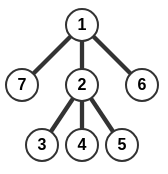
\includegraphics[height=100px]{sample-1-1}
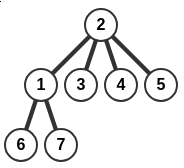
\includegraphics[height=100px]{sample-1-2}

Sehingga anggota nomor 1 punya 2 bawahan langsung maupun tidak langsung.

Pada kasus uji pertama, struktur anggota kerajaan mula-mula dapat digambarkan seperti gambar di bawah (kiri). Lalu, setelah anggota nomor 6 menjadi raja, struktur anggota kerajaan dapat digambarkan seperti gambar di bawah (kanan).

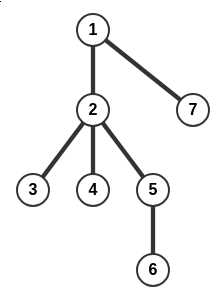
\includegraphics[height=150px]{sample-2-1}
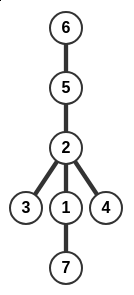
\includegraphics[height=150px]{sample-2-2}

Sehingga anggota nomor 2 punya 4 bawahan langsung maupun tidak langsung.


\end{document}